\documentclass{standalone}
\usepackage{tikz}

% == Tikz
\newcommand{\drawcirc}{\node[draw,circle,minimum size=1.5cm]}
\newcommand{\drawbox}{\node[draw,rectangle,minimum size=1.5cm]}
\newcommand{\drawdummy}{\node[minimum size=0,inner sep=0]}
\newcommand{\zeroSink}{\mathsf{o}}
\newcommand{\target}{\mathsf{f}}

\begin{document}
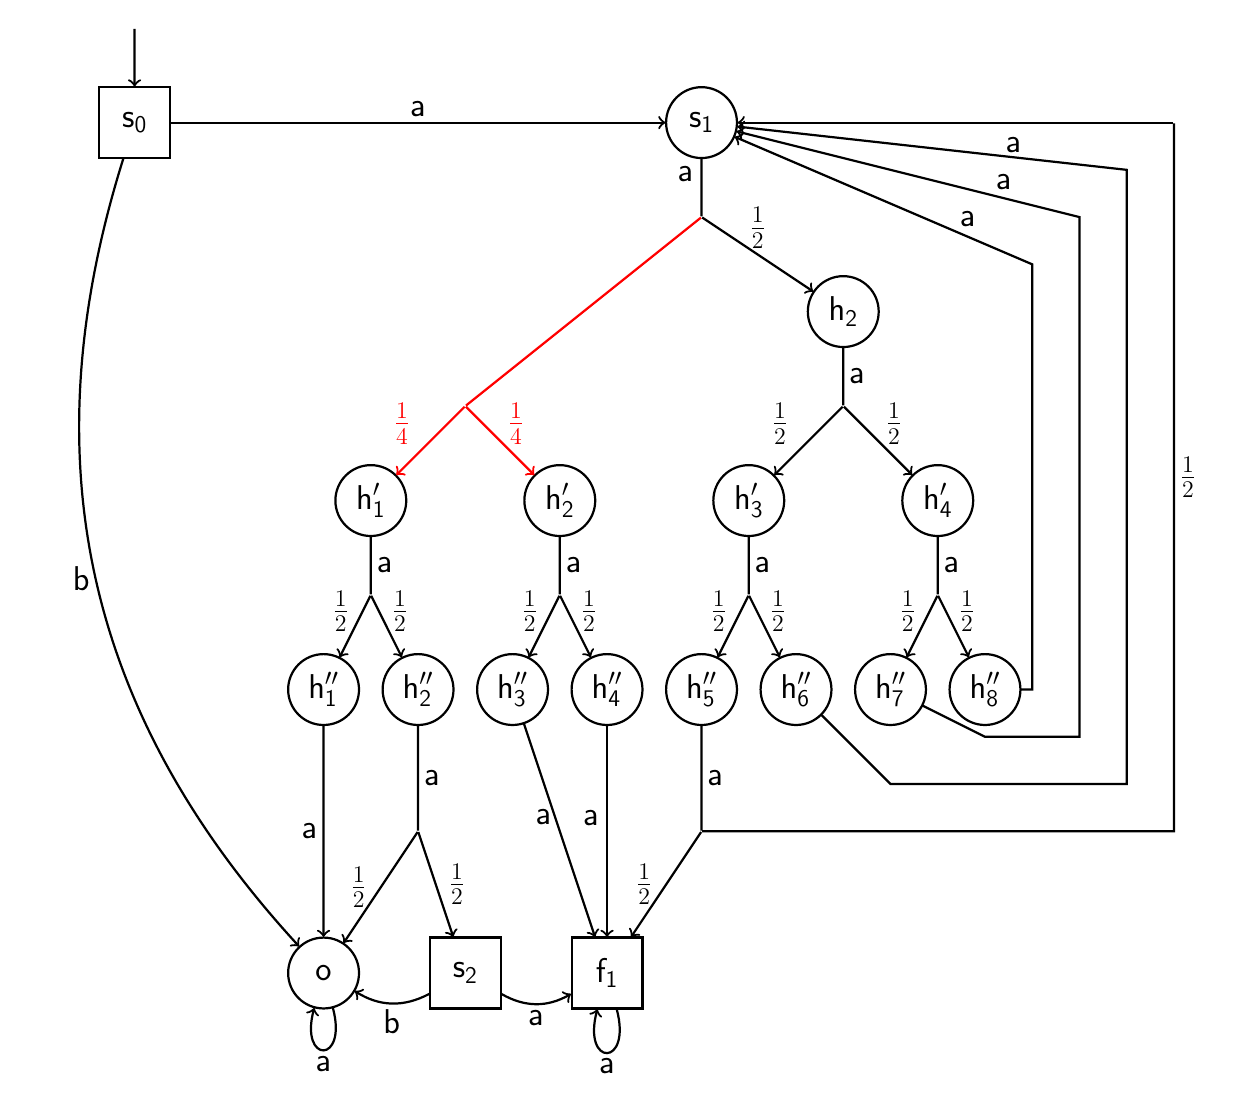
\begin{tikzpicture}[thick,scale=0.6, every node/.style={font=\huge, transform shape}]
%little BCEC with loop
\drawdummy (init) at (-8,2) {};
\drawbox (q) at (-8,0) {$\mathsf{s_0}$};
\drawcirc (p) at (4,0) {$\mathsf{s_1}$};
\drawdummy (mid) at (4,-2) {};
\drawbox (11) at (2,-18) {$\mathsf{f_1}$};
\drawbox (12) at (-1,-18) {$\mathsf{s_2}$};
\drawcirc (0) at (-4,-18)  {$\mathrm{\zeroSink}$};

\draw[->] (init) to (q);
\draw[->] (q) to node [above, midway] {$\mathsf{a}$}(p);
\draw[->] (q) to [bend right] node [left, midway] {$\mathsf{b}$}(0);

\draw[->] (0) to[loop below]  node [midway,below] {$\mathsf{a}$} (0);
\draw[->] (11) to [loop below] node [midway,below] {$\mathsf{a}$} (11);
\draw[->] (12) to [bend left] node [midway,below] {$\mathsf{b}$} (0);
\draw[->] (12) to [bend right] node [midway,below] {$\mathsf{a}$} (11);

\drawcirc (sHalf1) at (-4, -12) {$\mathsf{h_1''}$};
\drawcirc (sHalf2) at (-2, -12) {$\mathsf{h_2''}$};
\drawdummy (sHalf2Mid) at (-2, -15) {};
\drawcirc (sHalf3) at (0, -12) {$\mathsf{h_3''}$};
\drawcirc (sHalf4) at (2, -12) {$\mathsf{h_4''}$};
\drawcirc (sHalf5) at (4, -12) {$\mathsf{h_5''}$};
\drawdummy (sHalf5Mid) at (4, -15) {};
\drawdummy (sHalf5Help) at (14,0) {};
\drawcirc (sHalf6) at (6, -12) {$\mathsf{h_6''}$};
\drawcirc (sHalf7) at (8, -12) {$\mathsf{h_7''}$};
\drawcirc (sHalf8) at (10, -12) {$\mathsf{h_8''}$};

\draw[->] (sHalf1) to node [left, midway] {$\mathsf{a}$}(0);
\draw[-] (sHalf2) to node [right, midway] {$\mathsf{a}$}(sHalf2Mid);
\draw[->] (sHalf2Mid) to node [text width =0.5cm, midway, left] {$\frac{1}{2}$} (0);
\draw[->] (sHalf2Mid) to node [text width =-0.5cm, midway, right] {$\frac{1}{2}$} (12);

\draw[->] (sHalf3) to node [text width =1.0cm, above, midway] {$\mathsf{a}$}(11);
\draw[->] (sHalf4) to node [text width =1.0cm, above, midway] {$\mathsf{a}$}(11);

\draw[-] (sHalf5) to node [text width =1.0cm, right, midway] {$\mathsf{a}$}(sHalf5Mid);
\draw[->] (sHalf5Mid) to node [text width =0.5cm, midway, left] {$\frac{1}{2}$} (11);
\draw[-] (sHalf5Mid) to (14, -15)  to node [text width =0.5cm, midway, right] {$\frac{1}{2}$} (sHalf5Help);
\draw[->] (sHalf5Help) to (p);

\draw[->] (sHalf6) to (8, -14) to (13, -14) to (13, -1) to node [text width =1.0cm, above, near start] {$\mathsf{a}$}(p);
\draw[->] (sHalf7) to (10, -13) to (12, -13) to (12, -2) to node [text width = -0.1cm, above, near start] {$\mathsf{a}$}(p);
\draw[->] (sHalf8) to (11, -12) to (11, -3) to node [text width =-0.1cm, above, near start] {$\mathsf{a}$}(p);

\drawcirc (sLevelTwo1) at (-3, -8) {$\mathsf{h_1'}$};
\drawdummy (sLevelTwo1Mid) at (-3, -10) {};
\drawcirc (sLevelTwo2) at (1, -8) {$\mathsf{h_2'}$};
\drawdummy (sLevelTwo2Mid) at (1, -10) {};
\drawcirc (sLevelTwo3) at (5, -8) {$\mathsf{h_3'}$};
\drawdummy (sLevelTwo3Mid) at (5, -10) {};
\drawcirc (sLevelTwo4) at (9, -8) {$\mathsf{h_4'}$};
\drawdummy (sLevelTwo4Mid) at (9, -10) {};

\draw[-] (sLevelTwo1) to node [text width =1.0cm, right, midway] {$\mathsf{a}$}(sLevelTwo1Mid);
\draw[->] (sLevelTwo1Mid) to node [text width =0.5cm, near start, left] {$\frac{1}{2}$} (sHalf1);
\draw[->] (sLevelTwo1Mid) to node [text width =-0.5cm, near start, right] {$\frac{1}{2}$} (sHalf2);

\draw[-] (sLevelTwo2) to node [text width =1.0cm, right, midway] {$\mathsf{a}$}(sLevelTwo2Mid);
\draw[->] (sLevelTwo2Mid) to node [text width =0.5cm, near start, left] {$\frac{1}{2}$} (sHalf3);
\draw[->] (sLevelTwo2Mid) to node [text width =-0.5cm, near start, right] {$\frac{1}{2}$} (sHalf4);

\draw[-] (sLevelTwo3) to node [text width =1.0cm, right, midway] {$\mathsf{a}$}(sLevelTwo3Mid);
\draw[->] (sLevelTwo3Mid) to node [text width =0.5cm, near start, left] {$\frac{1}{2}$} (sHalf5);
\draw[->] (sLevelTwo3Mid) to node [text width =-0.5cm, near start, right] {$\frac{1}{2}$} (sHalf6);

\draw[-] (sLevelTwo4) to node [text width =1.0cm, right, midway] {$\mathsf{a}$}(sLevelTwo4Mid);
\draw[->] (sLevelTwo4Mid) to node [text width =0.5cm, near start, left] {$\frac{1}{2}$} (sHalf7);
\draw[->] (sLevelTwo4Mid) to node [text width =-0.5cm, near start, right] {$\frac{1}{2}$} (sHalf8);

%\node[red, draw,circle,minimum size=1.5cm] (sLevelOne1) at (-1, -4) {$\mathsf{h_1}$};
\drawdummy (sLevelOne1Mid) at (-1, -6) {};
\drawcirc (sLevelOne2) at (7, -4) {$\mathsf{h_2}$};
\drawdummy (sLevelOne2Mid) at (7, -6) {};

%\draw[red, -] (sLevelOne1) to node [text width =1.0cm, right, midway] {$\mathsf{a}$}(sLevelOne1Mid);
\draw[red, ->] (sLevelOne1Mid) to node [text width =1cm, near start, left] {$\frac{1}{4}$} (sLevelTwo1);
\draw[red, ->] (sLevelOne1Mid) to node [text width =-1cm, near start, right] {$\frac{1}{4}$} (sLevelTwo2);

\draw[-] (sLevelOne2) to node [text width =1.0cm, right, midway] {$\mathsf{a}$}(sLevelOne2Mid);
\draw[->] (sLevelOne2Mid) to node [text width =1cm, near start, left] {$\frac{1}{2}$} (sLevelTwo3);
\draw[->] (sLevelOne2Mid) to node [text width =-1cm, near start, right] {$\frac{1}{2}$} (sLevelTwo4);

\draw[-] (p) to node [text width =1.0cm, above, midway] {$\mathsf{a}$}(mid);
\draw[red, -] (mid) to (sLevelOne1Mid);
\draw[->] (mid) to node [midway, above] {$\frac{1}{2}$} (sLevelOne2);

\end{tikzpicture}
\end{document}
